\mode*
\section{Introduction}

\begin{frame}{Program Languages}
  \begin{block}{Machine code}
    The \alert{binary numbers} that the CPUs can understand.
    \begin{center}{\ttfamily
      100111000011101111001111 ... and so on ...}
    \end{center}
  \end{block}
  \begin{block}{Assembly language --- friendly to humans}
    People don't think in numbers.
    \begin{center}
      \mode<beamer>{ \includegraphics[width=.5\textwidth]{asm-sample-asm} }%
    \end{center}
    \mode<article>{ \includegraphics[width=.2\textwidth]{asm-sample-asm} }
    The ASM programs are translated to machine code by \alert{assemblers}.
  \end{block}
\end{frame}

\begin{frame}
  \begin{block}{High level languages}
    Even easier to understand for humans. Examples:
    \begin{itemize}
    \item C\tikzmark{clang}
    \item FORTRAN\tikzmark{fortran}
    \item Java\tikzmark{java}
    \item C++\tikzmark{cpp}
    \item ...\tikzmark{more}
    \end{itemize}\pause
    \alert{Compilers} do the translation work.    
  \end{block}
  \begin{tikzpicture}[remember picture,overlay,
    every node/.style={ellipse,red,opacity=.4,draw},
    every to/.style={append after command={[->,black!30,thick]}}
    ]
    \node (asm) at ($(pic cs:java) + (3,0)$) {Assembly};
    \node (bin) [right=of asm] {Binary};
    \draw ($(pic cs:clang)+(0,.5ex)$) to [bend left=20] (asm);
    \draw ($(pic cs:fortran)+(0,.5ex)$) to [bend left=15] (asm);
    \draw ($(pic cs:java)+(0,.5ex)$) to (asm);
    \draw ($(pic cs:cpp)+(0,.5ex)$) to [bend right=15] (asm);
    \draw ($(pic cs:more)+(0,.5ex)$) to [bend right=20] (asm);
    \draw (asm) to (bin);
    \end{tikzpicture}
\end{frame}

\begin{frame}{The History of C}
  \begin{description}
  \item[1967] \alert{BCPL} (Basic Computer Programming Language), Martin Richards
  \item[1970] \alert{B}, Bell Labs, Ken Thompson
  \item[1970+] \alert{C}, Bell Labs, Dennis Ritchie
  \item[1978] \alert{The C Programming Language}, B.Kernighan/D.Ritchie
  \item[1980] \alert{C++}, Bjarne Stroustrup
  \item[1989] \alert{ANSI C}, American National Standards Institute
  \item[1999] \alert{ISO/IEC 9899 C}, International Organisation for Standardization, 1999, the
    current Standard C
  \item[2000] \alert{C\#}, Anders Hejlsberg, Microsoft, 
  \end{description}
\end{frame}

\begin{frame}{Hello, world!}
  \begin{center}
    \mode<beamer>{ \includegraphics[width=.7\textwidth]{hello-c} }%
    \mode<article>{ \includegraphics[width=.3\textwidth]{hello-c} }
  \end{center}
  {\ttfamily
    \begin{itemize}
    \item[\$] edit hello.c
    \item[\$] gcc -Wall hello.c -o hello
    \item[\$] ./hello
    \end{itemize}}
\end{frame}

\begin{frame}{Toolchain}
\begin{center}
  \mode<beamer>{ 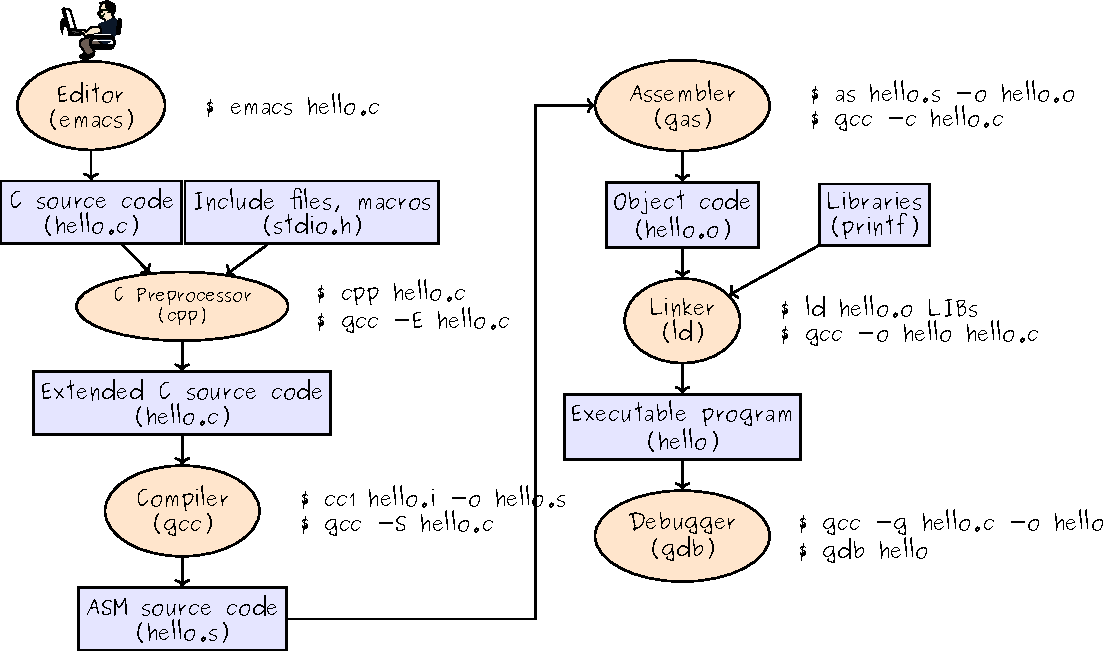
\includegraphics[width=\textwidth]{toolchain2} }%
  \mode<article>{ 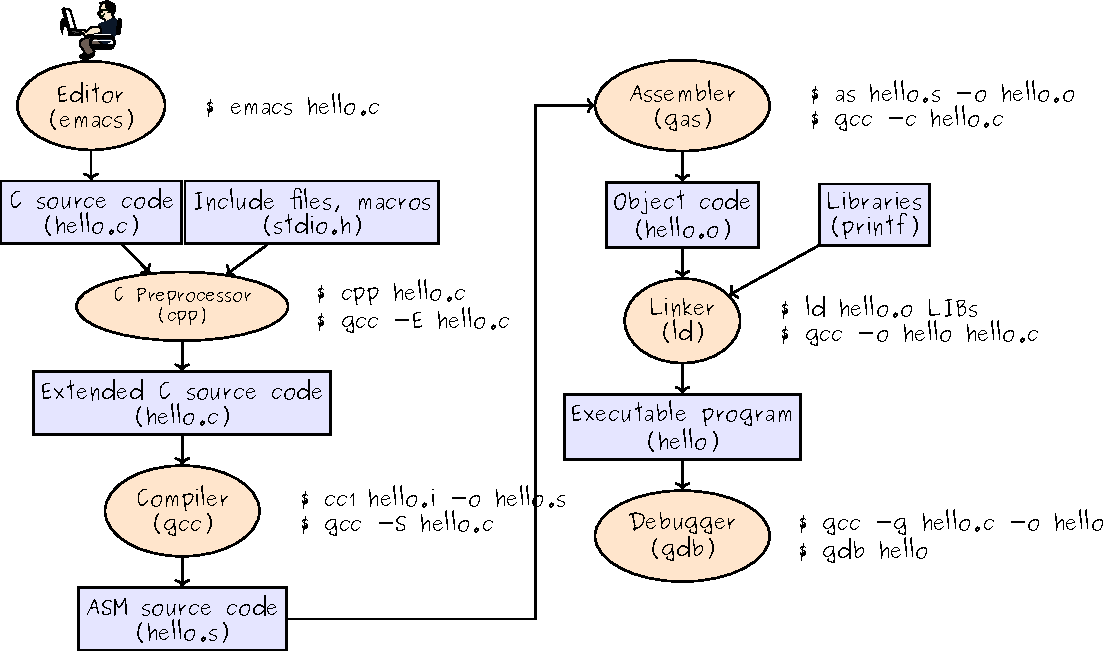
\includegraphics[width=.6\textwidth]{toolchain2} }
\end{center}
\end{frame}

\begin{description}
\item[Source code] written by programmer in high-level language, in our case in
  \texttt{C}. We write c source code with a \emph{text editor}, such as \texttt{emacs},
  \texttt{vim}, etc.
\item[Preprocessing] is the first pass of any C compilation. It processes
  \texttt{include-files}, \texttt{conditional compilation instructions} and
  \texttt{macros}.
  \begin{description}
  \item[cpp] The GNU C preprocessor
    \begin{itemize}
    \item[\$] \texttt{gcc -E hello.c}
    \end{itemize}
  \end{description}
\item[{Compilation}] is the second pass. It takes the output of the preprocessor, and the
  \texttt{source code}, and generates \texttt{assembly source code}.
  \begin{description}
  \item[gcc/g++] GNU C/C++ compiler
    \begin{itemize}
    \item[\$] \texttt{gcc -S hello.c}
    \end{itemize}
  \end{description}
\item[Assembly] is the third stage of compilation. It takes the assembly source code and
  produces an assembly listing with offsets. The assembler output is stored in an
  \texttt{object file}.
  \begin{description}
  \item[as] the portable GNU assembler
    \begin{itemize}
    \item[\$] \texttt{gcc -c hello.c}
    \end{itemize}
  \end{description}
\item[Linking] is the final stage of compilation. It combines object code with predefined
  routines from \texttt{libraries} and produces the \texttt{executable program}.
  \begin{description}
  \item[ld] The GNU linker
    \begin{itemize}
    \item[\$] \texttt{gcc hello.c -lm}
    \end{itemize}
  \end{description}
\item[{Wrapper}] The whole compilation process is usually not done `by hand', but using a
  \texttt{wrapper} program that combines the functions of preprocessor(cpp),
  compiler(gcc/g++), assembler(as) and linker(ld).
  \begin{itemize}
  \item[\$] \texttt{gcc -Wall hello.c -lm -o hello}
  \end{itemize}
\end{description}

See also: \href{http://www.tenouk.com/ModuleW.html}{COMPILER, ASSEMBLER, LINKER AND LOADER:
A BRIEF STORY}.\footnote{\url{http://www.tenouk.com/ModuleW.html}}

\mode<all>
%%% Local Variables:
%%% mode: latex
%%% TeX-master: "c-b"
%%% End:
